\section{Sơ đồ Lược đồ Logic}

Lược đồ dưới đây tương ứng với tập phụ thuộc hàm đã xét ở mục chuẩn hóa. Các ràng buộc miền giá trị và ràng buộc duy nhất bổ sung được trình bày ở từ điển dữ liệu.

Hệ thống tồn tại bốn mối kết hợp nhiều--nhiều đã được phân rã qua thực thể trung gian: quan hệ giữa \texttt{AppUser} và \texttt{Contest} phân rã qua \texttt{ContestRole}, quan hệ giữa \texttt{Entry} và giám khảo phân rã qua \texttt{ScoreSheet}, quan hệ giữa \texttt{ScoreSheet} và \texttt{Criterion} phân rã qua \texttt{ScoreDetail}, còn quan hệ đệ quy nghi trùng trên \texttt{EntryPhoto} phân rã qua \texttt{DuplicateMatch}.


\begin{figure}[H]
    \centering
        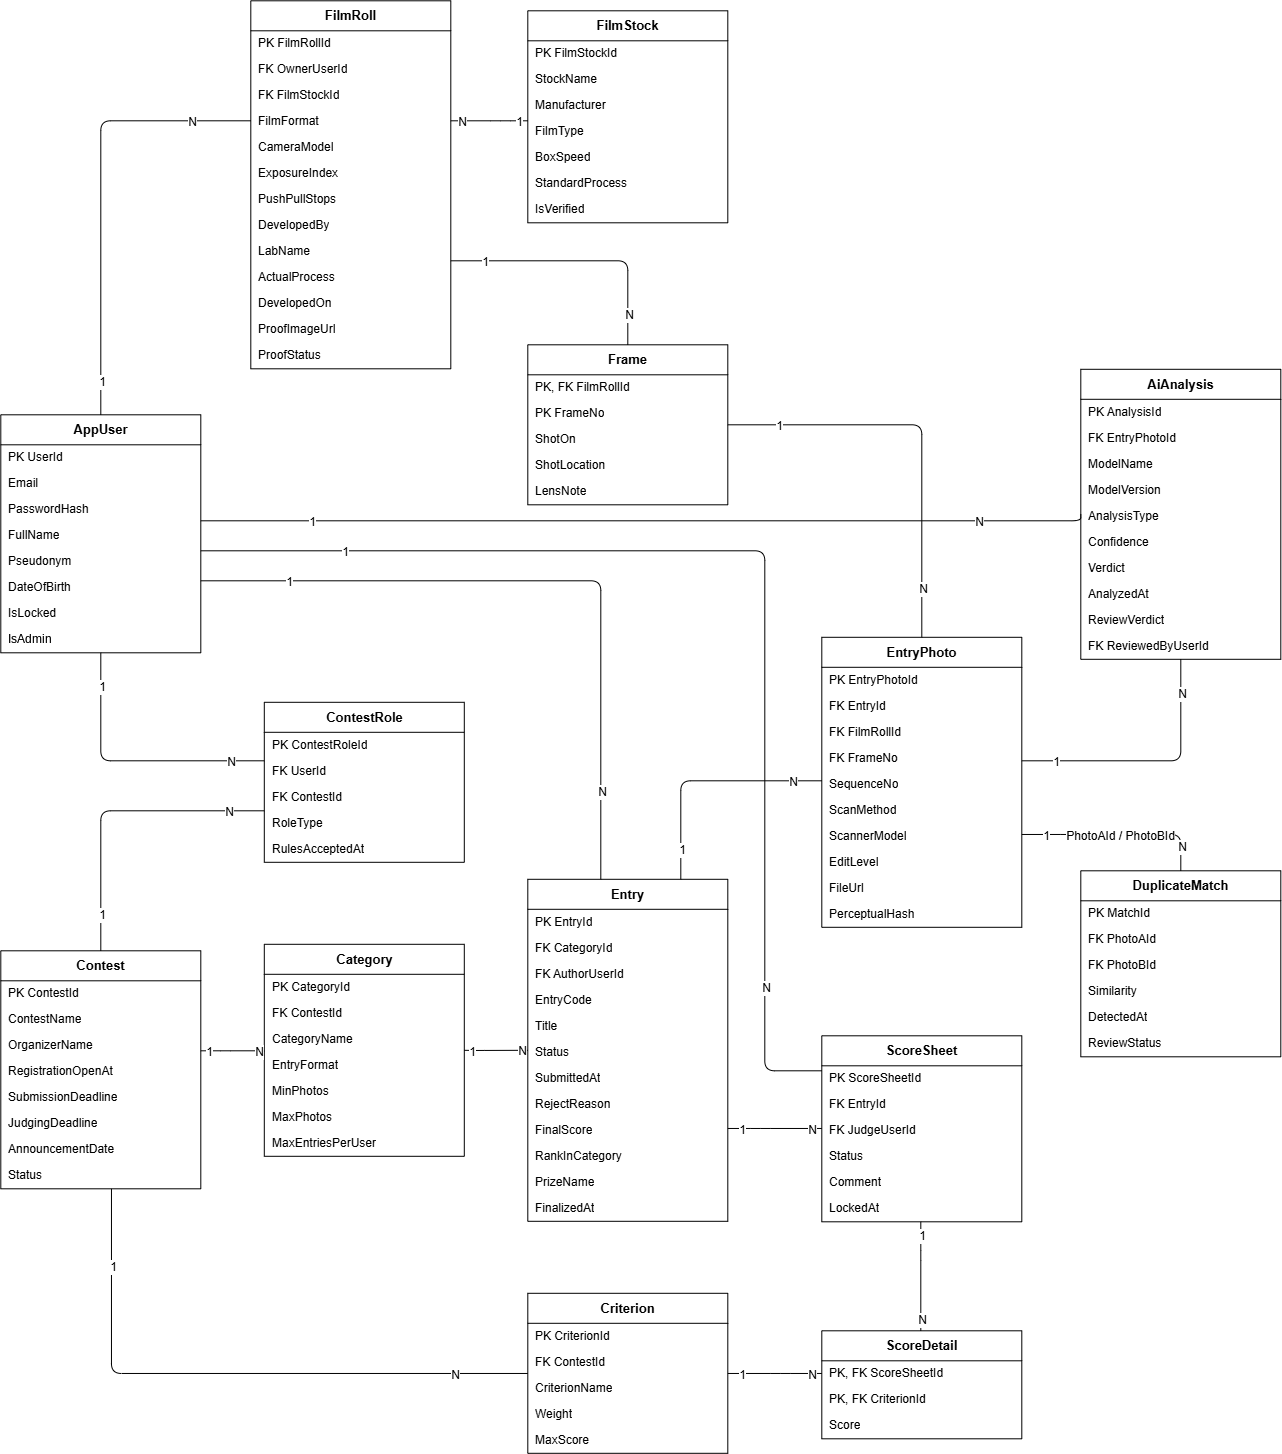
\includegraphics[width=\textwidth]{images/So_do_logic.png}
    \caption{Sơ đồ thiết kế logic (Logical Diagram)}
    \label{fig:3.1}
\end{figure}


